\section{Software Model}
\label{sec:softwareModel}

\subsection{Functional Requirements}

A Python model was constructed to provide a simulation of the movement and intersection of rays from a movable source to evaluate sensor performance and compare these results with practical experiments.
The model allows for a number of configurable parameters:
\begin{itemize}
    \item Trajectory of the light source in 3D space, which moves in configurable discrete increments.
    \item Placement, dimensions, and quantity of any number of sensors and apertures.
    \item Output visualisation, as a static, or animated graphic.
\end{itemize}
Affording flexibility for the model to simulate any sensor topology under a variety of conditions.

\begin{figure}[htbp] %h-ere t-op b-ottom p-page (separte) -good to allow all htbp to give the compiler more options
    \centering
    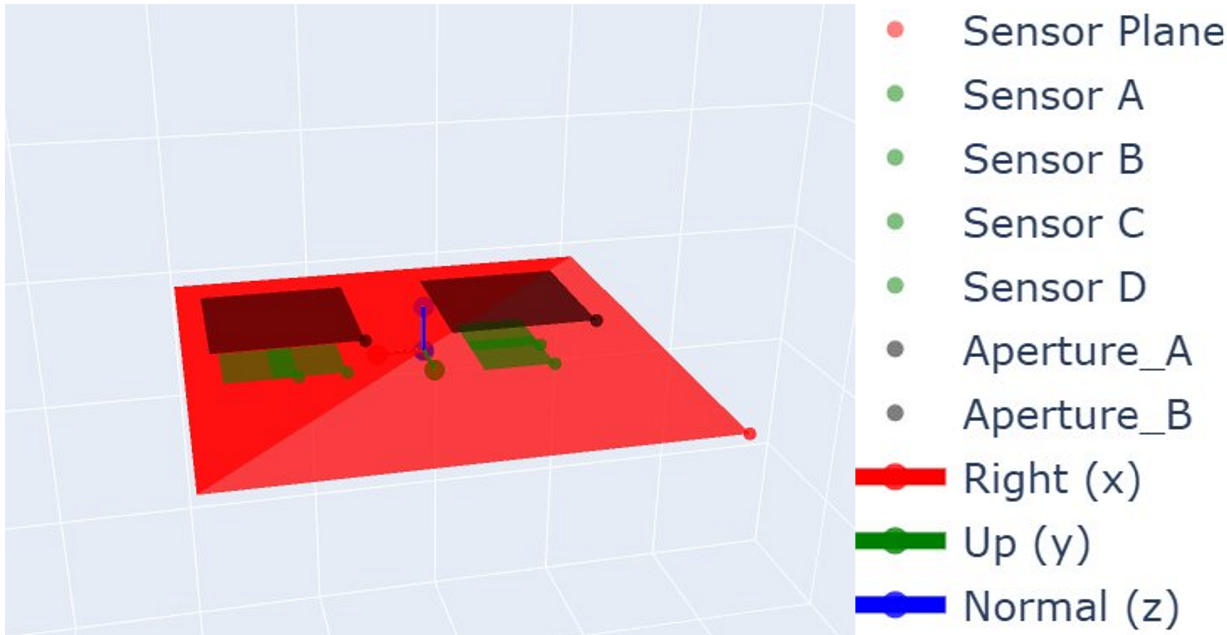
\includegraphics[width=0.8\textwidth]{chapters/methodology/SoftwareModel/images/Sensor plane.png} % change {path}
    \caption{Sensor Toplogy}       % change {caption}
    \label{fig:Sensor Topology}            % change label - used for reference in text
\end{figure}                             % for example: see in Figure~\ref{example label}


% State the theory
\subsection{Theory and Concept}
In order to encapsulate the real life behaviours required to simulate this system, the software model is designed to around a structure based on the classes “Planes”, “Areas”, and “Lines”. These classes contain methods related to each of their properties and stores data on their states.    

% Ray projection
The basis for the 3D geometry involves defining:
\begin{itemize}
    \item Each line by vectors representing position and normal direction, $ \vec{A} = (a,b,c)$ and $ \vec{u} = (\alpha, \beta, \gamma)$
    \item Each plane by the vectors $\vec{P} = (l,m,n) $ and $ \vec{n} = (\lambda, \mu, \nu)$, respectively.
\end{itemize}

\subsubsection{Coordinate System}

Each ray is initially defined in the local coordinate system of the source plane. This local frame is established by three orthonormal basis vectors:

\begin{itemize}
    \item $\vec{r}$ — right vector (local $x$-axis)
    \item $\vec{u}$ — up vector (local $y$-axis)
    \item $\vec{n}$ — normal vector (local $z$-axis)
\end{itemize}

These vectors form the columns of a rotation matrix $R$ which transforms local coordinates to global:

\begin{equation}
R = 
\begin{bmatrix}
\vec{r} & \vec{u} & \vec{n}
\end{bmatrix}
=
\begin{bmatrix}
r_x & u_x & n_x \\
r_y & u_y & n_y \\
r_z & u_z & n_z \\
\end{bmatrix}
\label{eq:rotation_matrix}
\end{equation}

A point $\vec{p}_\text{local} = \begin{bmatrix} x_l & y_l & z_l \end{bmatrix}^\top$ defined in local coordinates is converted to global coordinates via:

\begin{equation}
\vec{p}_\text{global} = \vec{p}_\text{plane} + R \cdot \vec{p}_\text{local}
\label{eq:local_to_global}
\end{equation}

Where:
\begin{itemize}
    \item $\vec{p}_\text{plane}$ is the global position of the origin of the plane
    \item $R$ rotates the local point into the global frame
\end{itemize}

This ensures that all rays originating from the source plane move coherently when the plane is rotated or translated.

\subsubsection{Ray generation}
Rays are randomly generated within the bounds of the source plane, whose position, size, and direction are defined in the configuration. The position of each ray is calculated using:

% Ray generation equation
\begin{equation}
X_i \sim \mathcal{U}\left(-\frac{w}{2}, \frac{w}{2}\right), \quad
Y_i \sim \mathcal{U}\left(-\frac{l}{2}, \frac{l}{2}\right), \quad
\text{for } i = 1, \ldots, N
\label{eq:RayGeneration}
\addequation{Ray Generation}
\end{equation}

Ray projection, from a source plane to a sensor plane, is modelled using the parametric equation of a 3D line (\ref{eq:ray_projection}). This allows each ray to be described in terms of a parameter $t$, which enables the calculation of the intersection points between the light rays and the sensor plane. 

\subsubsection{Line-Plane Intersection}
% Intersection equation
\begin{equation}
\frac{x - a}{\alpha} = \frac{y - b}{\beta} = \frac{z - c}{\gamma} (=t)
\label{eq:ray_projection}
\addequation{Ray projection}
\end{equation}

Where the intersection coordinates $(x,y,z)$ occur within a target area, a hit occurs, representing illumination.

For any given combination of source plane, and sensor plane, the $t$ parameter is calculated using the Line-Plane Intersection equation.

\begin{equation}
    t = \frac{\vec{n} \cdot \vec{P} - \vec{n} \cdot \vec{A}}{\vec{n} \cdot \vec{u}}
    \label{eq:Line_Plane_Intersection}
\end{equation}
% comment

\subsubsection{Arc movement}
% Arc movement
The simulation converts between spherical (polar) and Cartesian coordinate systems to define the movement of the source plane along an arc trajectory. This transformation enables position and orientation of the plane in 3D. 

The spherical coordinates are expressed as ($r, \theta, \varphi$) and are converted to Cartesian as:
\begin{align}
x &= r \cdot \sin(\varphi) \cdot \cos(\theta) \\
y &= r \cdot \sin(\varphi) \cdot \sin(\theta) \\
z &= r \cdot \cos(\varphi)
\end{align}

This enables generation of plane positions around a defined arc, supporting vertical, horizontal, and rigid trajectory configurations.

\paragraph{Movement types}
\begin{itemize}
    \item Azimuthal Scanning / Vertical Circles: The azimuthal angle $\theta$ remains fixed, while the elevation angle $\varphi$ is varied. 
    \item Polar Scanning / Horizontal Circles: The elevation angle $\varphi$ remains fixed, while the azimuthal angle $\theta$ is varied. 
    \item Rigid Arc: A semi-circlular path in the $xz-plane$ is generated, with the plane rigidly rotated to always face the origin. This mode uses the Rodrigues rotation formula to reorient the source plane toward the target, as it required rotation about an arbitary axis.  
\end{itemize}

\begin{equation}
R = I + \sin\theta \cdot K + (1 - \cos\theta) \cdot K^2
\label{eq:RodriguesMatrix}
\addequation{Rodrigues Rotation Formula Matrix}
\end{equation}
\begin{equation}
K = 
\begin{bmatrix}
0 & -k_z & k_y \\
k_z & 0 & -k_x \\
-k_y & k_x & 0
\addequation{Skew-symmetric matrix}
\end{bmatrix}
\end{equation}

For each position along the trajectory, the plane is rotated such that its normal direction vector $\vec{n}$ points towards to the origin, about which the sensor plane is defined.  

\begin{table}[H]
\centering
\caption{Definition of vectors and symbols used in ray and plane calculations}
\label{tab:symbols}
\begin{tabular}{ll}
\toprule
\textbf{Symbol} & \textbf{Description} \\
\midrule
$\vec{A} = (a, b, c)$ & Position vector of the ray origin \\
$\vec{u} = (\alpha, \beta, \gamma)$ & Direction vector of the ray \\
$\vec{P} = (l, m, n)$ & A known point on the target plane \\
$\vec{n} = (\lambda, \mu, \nu)$ & Normal vector of the target plane \\
$t$ & Ray parameter defining point along the ray path \\
$r$ & Radius in spherical coordinates \\
$\theta$ & Azimuthal angle in spherical coordinates \\
$\varphi$ & Elevation angle in spherical coordinates \\
\bottomrule
\end{tabular}
\end{table}
% State the theory
\subsection{Implementation}

The software model implements the theoretical foundation to provide a flexible framework for simulating ray projection and intersection calculations. The implementation follows a modular object-oriented approach with  components that can be configured to represent different experimental setups.

\subsubsection{Architecture Overview}

The architecture consists of several key components:
\begin{itemize}
\item Core geometric objects (Planes, Areas, Lines) that encapsulate the mathematical properties
\item Simulation engine for trajectory generation and intersection testing
\item Configuration system for experiment setup
\item Visualisation  pipeline for result analysis
\item User interface for interactive control
\end{itemize}

\subsubsection{Model Configuration}

A .JSON file is used to allow for easy setup of different experimental scenarios without modifying code:

\begin{itemize}
\item Detailed definition of planes, including position, orientation, and dimensions
\item Sensor and aperture areas with specific positions and sizes
\item Trajectory specifications for various movement types
\item Simulation parameters (number of rays, iterations)
\item Visualisation options - Static, or animated plot 
\item Debugging and performance settings
\end{itemize}

The \texttt{Config} class (Listing~\ref{lst}) loads and parses the configuration file, making parameters accessible throughout the application:
\begin{lstlisting}[style=pythonstyle, caption=Model configuration - Config Class, label=lst:pythonCodeApp, language=Python ]
    
    class Config:
        def init(self, file_path=None, data=None):
        if data is not None:
        self.load_from_dict(data)
        elif file_path:
        with open(file_path, "r") as f:
        data = json.load(f)
        self.load_from_dict(data)
        else:
        raise ValueError("Must provide either file_path or data")
    
    def load_from_dict(self, data):
        self.planes = data["planes"]
        self.sensor_areas = data["sensor_areas"]
        self.aperture_areas = data["aperture_areas"]
        self.arc_movement = data["arc_movement"]
        self.simulation = data["simulation"]
        self.intersection = data["intersection"]
        self.visualization = data["visualization"]
        self.debugging = data["debugging"]
        self.performance = data["performance"]
        self.output = data["output"]
    \end{lstlisting}
\subsection{Data Analysis and Evaluation}
After the ray-tracing simulation completes, the data generated is analysed to evaluate the performance of the sensor topology. 

This component evaluates the performance of the system at each step along the trajectory of the source plane. The analysis uses data stored in the $results-\\.csv$ and $sensor\_results.csv$ output files to calculate and visualise hit efficiency. 

\subsubsection{Result Analysis Function: \texttt{plot\_hit\_percentage()}}

This script evaluates the system’s ray interception efficiency across the arc rotation of the source plane, generating two plots:

\paragraph{\textbf{Overall Hit Percentage per Arc Index}}

This plot displays the proportion of emitted rays that successfully reach any of the defined sensor areas for each simulation index (arc position). The hit percentage is calculated as:
\begin{equation}
    \text{Hit (\%)} = \frac{\text{Number of Hits}}{\text{Total Number of Rays}} \times 100
    \label{eq:Overall_Hit_Percentage}
    \addequation{Overall Hit Results (\%)}
    \end{equation}

\paragraph{\textbf{Per-Sensor Hit Percentage}}
Gaining spatial resolution of the intersection behaviours, the second subplot shows the relative 'illumination' of each sensor based on the total hits. For every arc index, the number of rays detected by each sensor is normalised by the total number of hits. This allows identification of the directional coverage for each sensor. 

\begin{figure}[htbp] %h-ere t-op b-ottom p-page (separte) -good to allow all htbp to give the compiler more options
    \centering
    \includegraphics[width=0.8\textwidth]{chapters/methodology/SoftwareModel/images/plot\_hit\_percentage\_combined.png} % change {path}
    \caption{\texttt{plot\_hit\_percentage()} Output Plot}       % change {caption}
    \label{fig:Hit Percentage Output Plot}            % change label - used for reference in text
\end{figure}                             % for example: see in Figure~\ref{example label}

\vspace{1em}
Together these visualisations form an overview of the sensor system's performance and directional sensitivity. 

\subsubsection{Sensor Spatial Response Function: \texttt{sensor\_surface\_plots()}}
While previous analysis plots visualise results per arc index, this function presents a higher-dimensional insight by mapping each sensor’s illumination response across both the arc angle and the tilt angle. The underlying data is drawn from \texttt{sensor\_results.csv} and the angular mapping in \texttt{rigid\_arc\_angles.csv}.

Each output is a 3D surface plot, Figure~\ref{fig:Sensor Surface Output Plot}, where:
\begin{itemize}
    \item The $x$-axis represents the \textbf{arc angle} (horizontal angular sweep),
    \item The $y$-axis represents the \textbf{tilt angle} (vertical angular sweep),
    \item The $z$-axis shows the \textbf{number of ray hits} for each sensor.
\end{itemize}
This visualisation allows for an evaluation of the angular coverage of each sensor and the orthogonality of the measurements.
\begin{landscape}
    \begin{figure}[p] %h-ere t-op b-ottom p-page (separte) -good to allow all htbp to give the compiler more options
        \centering
        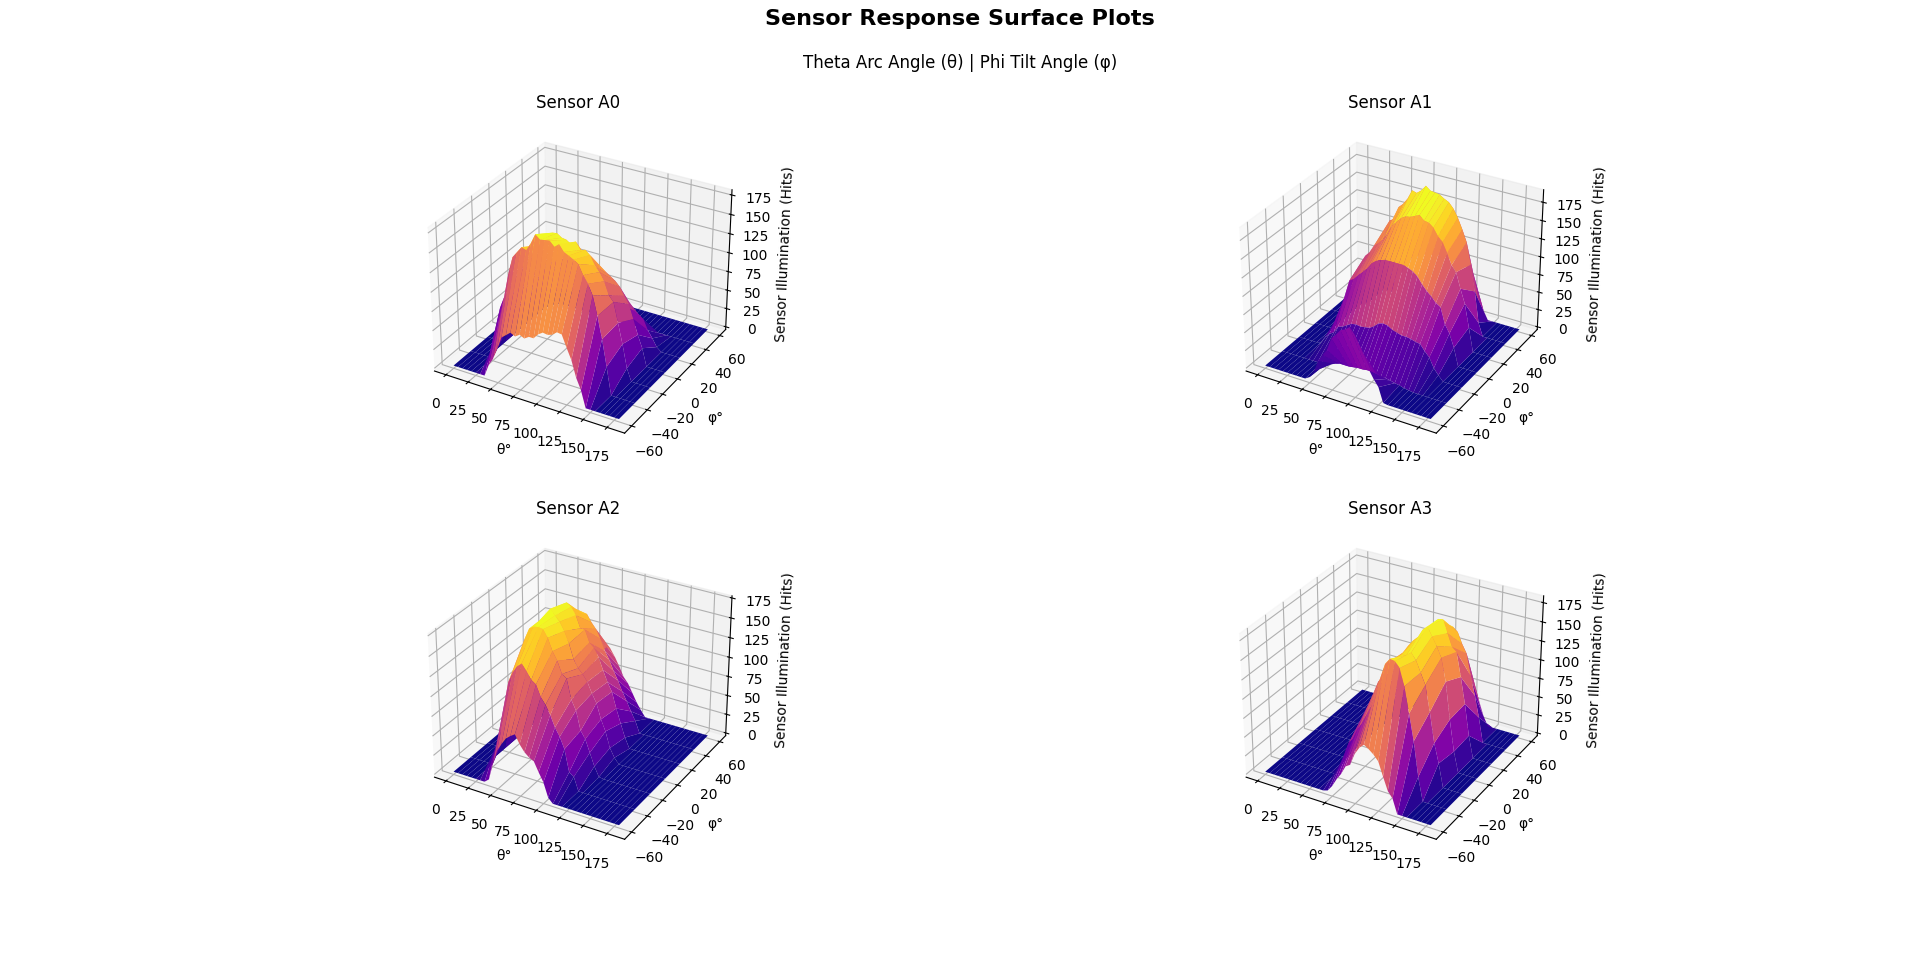
\includegraphics[width=1\textwidth]{chapters/methodology/SoftwareModel/images/Sensor Surface Plots.png} % change {path}
        \caption{\texttt{sensor\_surface\_plots()} Output Plot}       % change {caption}
        \label{fig:Sensor Surface Output Plot}            % change label - used for reference in text
    \end{figure}
\end{landscape}

\subsubsection{Model Testing}
To validate the functionality of the model test configurations were created. Each test scenario targets a specific feature or behaviour of the ray-plane interaction system, ensuring that the model behaves as expected.

The simulation framework was tested using several `.json` configuration files, each defining different spatial setups for the source, aperture, and sensor planes. The expected outcome of each test was determined analytically based on geometric relationships. Below is a summary of each test and its intended validation purpose:

\begin{itemize}
    \item \textbf{test\_arc\_rotation.json} \\
    This test evaluates the full arc movement of the source plane in a rigid semi-circular path, with multiple sensors and two distinct apertures. The simulation checks whether rays, emitted from various arc positions, are correctly filtered through the apertures and accurately detected by the sensors. \textit{Expected result:} a non-uniform distribution of sensor hits across arc positions, demonstrating correct handling of dynamic source movement and occlusion logic.
    
    \item \textbf{test\_directly\_below.json} \\
    A basic validation scenario where a single sensor is placed directly beneath a uniformly open aperture and source. The system is expected to demonstrate maximal efficiency under ideal alignment conditions. \textit{Expected result:} High \% ray intersection success with the sensor area.

    \item \textbf{test\_no\_intersection.json} \\
    This test ensures that rays that are directed orthogonally to the sensor plane (i.e., no downward component). The source emits horizontally, and the sensor is placed far from the expected ray path. \textit{Expected result:} zero valid intersections, confirming non-intersection conditions.

    \item \textbf{test\_off\_center.json} \\
    In this configuration, sensors are slightly offset from the central axis of the source, with a wide aperture. This test is used to assess the spatial precision of the system when determining ray hits that fall near sensor boundaries. \textit{Expected result:} a partial detection pattern, with hits concentrated on central sensors and misses on outer ones depending on angular spread.

    \item \textbf{test\_with\_aperture.json} \\
    This test includes two apertures spatially separated along the y-axis and a single sensor aligned with one of them. It is intended to verify whether rays are correctly filtered by the aperture before reaching the sensor. \textit{Expected result:} Most rays intersect outside aligned apertures, with sensor registering hits only through valid aperture intersecting paths.

\end{itemize}

Together, these tests provide functional validation of the core components: ray generation, source arc trajectory, aperture filtering, and intersection logic. The system’s ability to handle edge cases (e.g., no intersection, misalignment) supports its robustness and practical viability for analysis and experimentation of potential sensor topologies.

\subsubsection{Model Evaluation Function: \texttt{Run Time and Hit Gain Efficiency}}

The second aspect focuses on the computational performance of the simulation in relation to the effects of increasing the number of rays.
This is implemented in the $plot\_runtime\_vs\_gain()$ function, which processes $results.csv$ to compute:

\paragraph{\textbf{Average Runtime per Ray Count}}

- The mean execution time required for the simulation of varying ray counts, providing a baseline for understanding the simulation's computational demands.

\paragraph{\textbf{Marginal Gain in Hit Percentage}}
- This quantifies how much additional hit accuracy is gained by increasing the number of rays. It is computed by taking the difference in hit percentage between successive ray counts. This helps to identify the point(s) of diminishing returns, where increasing the ray count leds to diminishing returns in terms of accuracy.

\paragraph{\textbf{Cost per Percentage Gain}}
- Further quantifying efficiency, this analysis calculates the cost per 1\% gain in hit percentage. This expresses how many seconds of simulation time are required to improve accuracy by one percentage point, it provides insight into whether it is computationally justified to increase ray count. 

\begin{equation}
    \text{Cost per Gain} = \frac{\Delta \text{Runtime}}{\Delta \text{Hit Percentage}}
    \label{eq:Cost_per_Gain}
    \addequation{Cost per Gain accuracy}
\end{equation}

\vspace{1em}


\begin{figure}[htbp] %h-ere t-op b-ottom p-page (separte) -good to allow all htbp to give the compiler more options
    \centering
    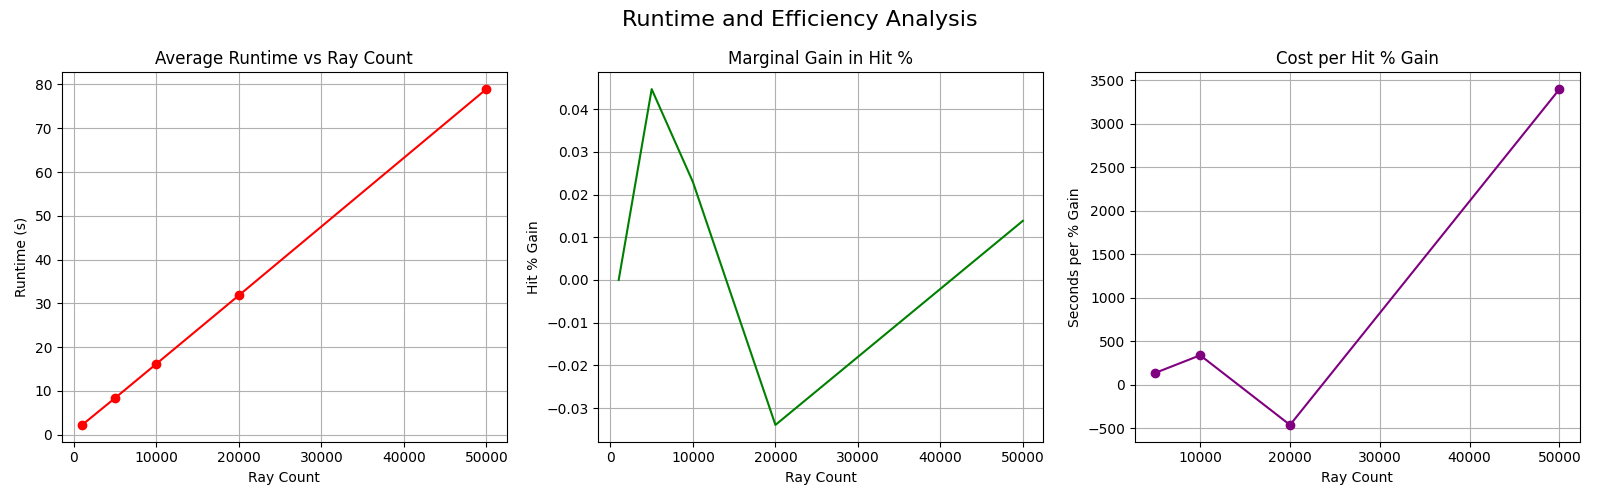
\includegraphics[width=0.9\textwidth]{chapters/methodology/SoftwareModel/images/run time analysis.png} % change {path}
    \caption{\texttt{Run Time and Hit Gain Efficiency} Output Plot}       % change {caption}
    \label{fig:Run Time and Hit Gain Efficiency}            % change label - used for reference in text
\end{figure}  

These results help in determining the optimal ray count against computational expense, ensuring that the simulation remains accuracy and practical.



    \begin{table}[h]
        \centering
        \caption{Summary of Analysis Functions}
        \label{tab:analysis_summary}
        \begin{tabular}{>{\raggedright}p{4cm} >{\raggedright}p{5cm} >{\raggedright\arraybackslash}p{5cm}}
            \toprule
            \textbf{Function} & \textbf{Metrics Generated} & \textbf{Purpose} \\
            \midrule
            \texttt{plot\_hit\_percentage \_combined()} & Overall Hit Percentage \newline Per-Sensor Hit Distribution & Assess ray interception performance and directional sensitivity \\
            \texttt{plot\_runtime\_vs \_gain()} & Average Runtime \newline Marginal Gain in Hit \% \newline Cost per Gain & Evaluate efficiency vs. accuracy trade-offs in ray count configuration \\
            \texttt{sensor\_surface \_plots()} & Sensor Response 3D Surfaces & Visualise angular response behaviour of each sensor across the full tilt/arc space \\
            \bottomrule
        \end{tabular}
    \end{table}

\subsection{Model Results}

\subsubsection{Runtime and Efficiency Analysis}

To evaluate the computational efficiency of the simulation model, a series of runs were performed using increasing ray counts. The aim was to determine how runtime scales with simulation complexity, and whether additional rays meaningfully improve hit accuracy.

\begin{figure}[H]
    \centering
    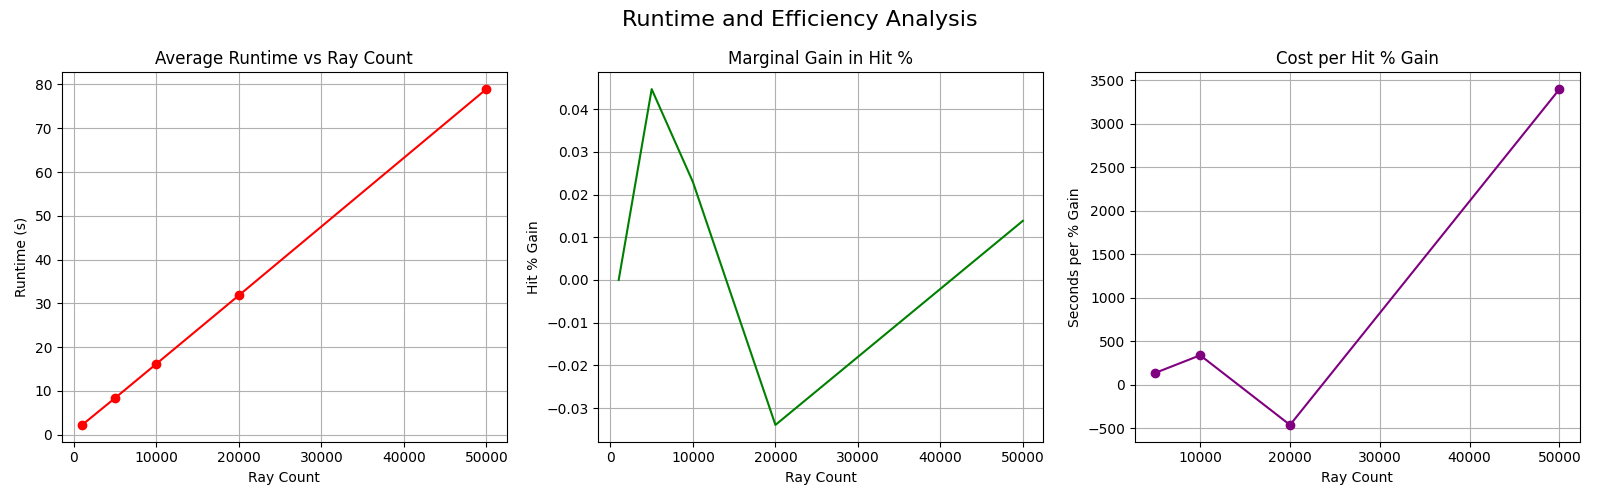
\includegraphics[width=\textwidth]{chapters/methodology/SoftwareModel/images/run time analysis.png}
    \caption{Runtime and efficiency trends with increasing ray count. Left: Runtime increases linearly with ray count. Middle: Marginal gain in hit accuracy. Right: Cost in seconds per 1\% hit gain.}
    \label{fig:runtime_efficiency}
\end{figure}

\textbf{Scalability}: As shown in Figure~\ref{fig:runtime_efficiency} (left), the simulation runtime increases approximately linearly with the number of rays. This behaviour suggests the implementation scales efficiently.

\textbf{Accuracy vs. Rays}: The centre plot illustrates the marginal gain in hit percentage between successive ray counts. Gains were most meaningfully prominent between 20,000 and 50,000 rays.

\textbf{Cost per Gain}: The rightmost plot quantifies computational cost per 1\% gain in accuracy. It reveals that simulations using 50,000 rays are inefficient: they incur high runtimes with negligible improvement. In contrast, ray counts between 10,000 and 20,000 yield the most cost-effective results.

\textbf{Utilisation}: Based on these findings, simulations were conducted using \textbf{15,000 rays} to benefit from the best trade-off between runtime and accuracy.


